\documentclass[aspectratio=43]{beamer}
%Information to be included in the title page:
\title{Paper Reading}
\author{Dachun Kai}
\institute{USTC}
\date{October 18, 2021}
%\usetheme{CambridgeUS}
\usetheme{Boadilla}

\usepackage[backend=bibtex,sorting=none]{biblatex}
%\usepackage{ctex}
\addbibresource{ref.bib} %BibTeX数据文件及位置
\setbeamerfont{footnote}{size=\tiny}
\usepackage{graphicx}
\usepackage{animate}
\usepackage{hyperref}


\begin{document}
	\frame{\titlepage}
	
	\begin{frame}{XVFI\textit{(ICCV2021, Oral)}}
		\begin{figure}
			\centering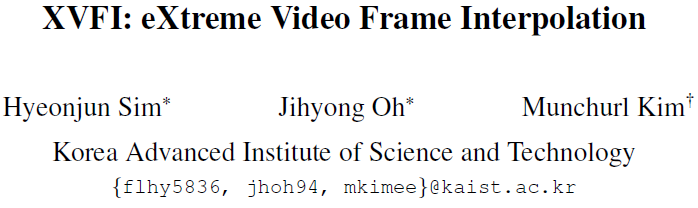
\includegraphics[width=0.75\linewidth]{images/title.png}
		\end{figure}
	\end{frame}

	\begin{frame}{Task: Video Frame Interpolation}
	\only<1>{
		\begin{itemize}
			\item A \alert{low-level} vision task to increase frame rate of a video.
			\item Method: \alert{motion-based}, kernel-based, phase-based, \alert{event-based}
			\item \alert{Flow-based} method framework:
		\end{itemize}
		\begin{figure}
			\centering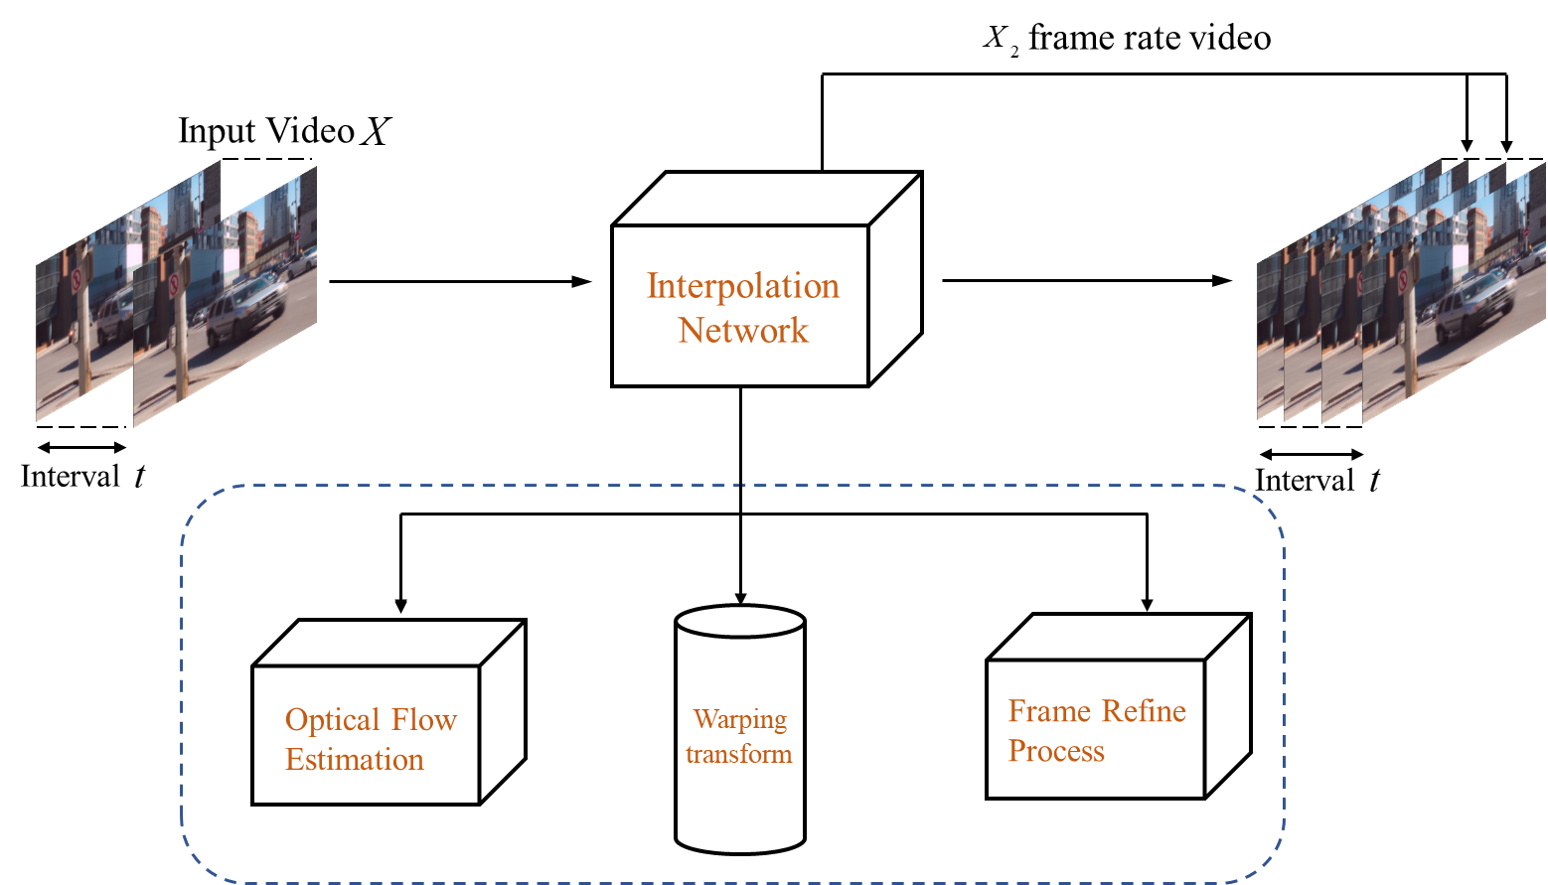
\includegraphics[width=0.7\linewidth]{images/inter_framework.png}
		\end{figure}
		\begin{itemize}
			\item Evaluation metric: \textit{PSNR}, \textit{SSIM}, \textit{IE}(Interpolation Error)
		\end{itemize}
		}
	\end{frame}

	\begin{frame}{Preliminaries: Optical Flow and Backward Warping}
		\begin{itemize}
			\item Optical Flow depicts \alert{motion} of objects in a visual scene.
		\end{itemize}
		\begin{figure}
			\centering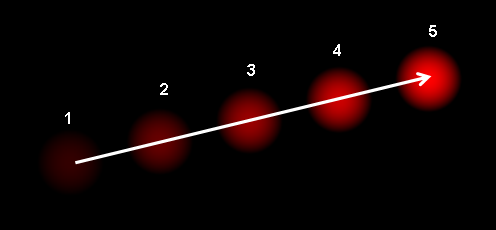
\includegraphics[width=0.4\linewidth]{images/Optical_flow_example.png}
		\end{figure}
		\begin{itemize}
			\item Flow Example:
		\end{itemize}
		\begin{figure}
			\centering
			\animategraphics[loop, autoplay, width=0.8\linewidth]{20}{./images/temp/temp}{1}{110}
		\end{figure}
		\begin{itemize}
			\item Image Warping
		\end{itemize}
		\begin{figure}
			\centering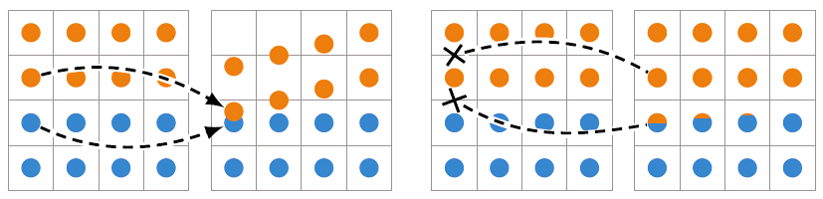
\includegraphics[width=0.6\linewidth]{images/warping.png}
		\end{figure}
	\end{frame}

	\begin{frame}{Milestone: Super SloMo\footfullcite{jiang2018super}}
		\begin{figure}
			\centering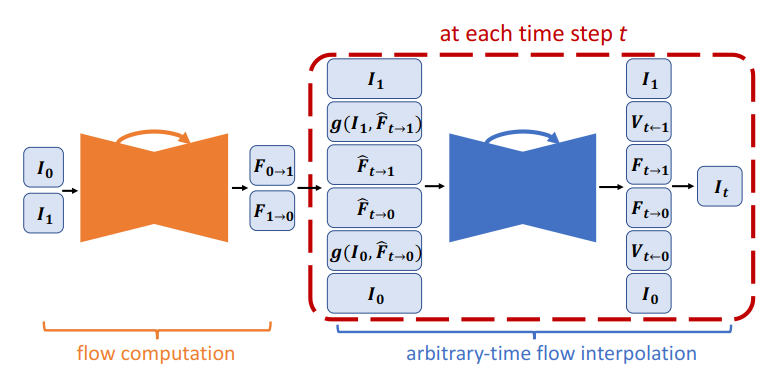
\includegraphics[width=0.7\linewidth]{images/smm.png}
		\end{figure}
		\begin{block}{Ideas}
			$$
			\begin{aligned}
			&\hat{F}_{t \rightarrow 0}=-(1-t) t F_{0 \rightarrow 1}+t^{2} F_{1 \rightarrow 0} \\
			&\hat{F}_{t \rightarrow 1}=(1-t)^{2} F_{0 \rightarrow 1}-t(1-t) F_{1 \rightarrow 0}
			\end{aligned}
			$$
			$$
			\hat{I}_{t}=\frac{1}{Z} \odot\left((1-t) V_{t \leftarrow 0} \odot g\left(I_{0}, F_{t \rightarrow 0}\right)+t V_{t \leftarrow 1} \odot g\left(I_{1}, F_{t \rightarrow 1}\right)\right)
			$$
		\end{block}
	\end{frame}

	\begin{frame}{Problem Definition}
		\begin{itemize}
			\item Motivation
			\begin{itemize}
				\item Handle the VFI for $4K$ videos with large motion, computed by IRR\footfullcite{hur2019iterative}.
			\end{itemize} 
		\end{itemize}
		\begin{figure}
			\centering
			\animategraphics[loop, autoplay, width=0.85\linewidth]{20}{./images/motion/temp}{1}{154}
		\end{figure}

	\end{frame}

	\begin{frame}{Proposed X4K1000FPS Dataset}
		\only<1>{
		\begin{itemize}
			\item Impressive \alert{$4K@1000fps$} dataset.
		\end{itemize}
		\begin{figure}
			\centering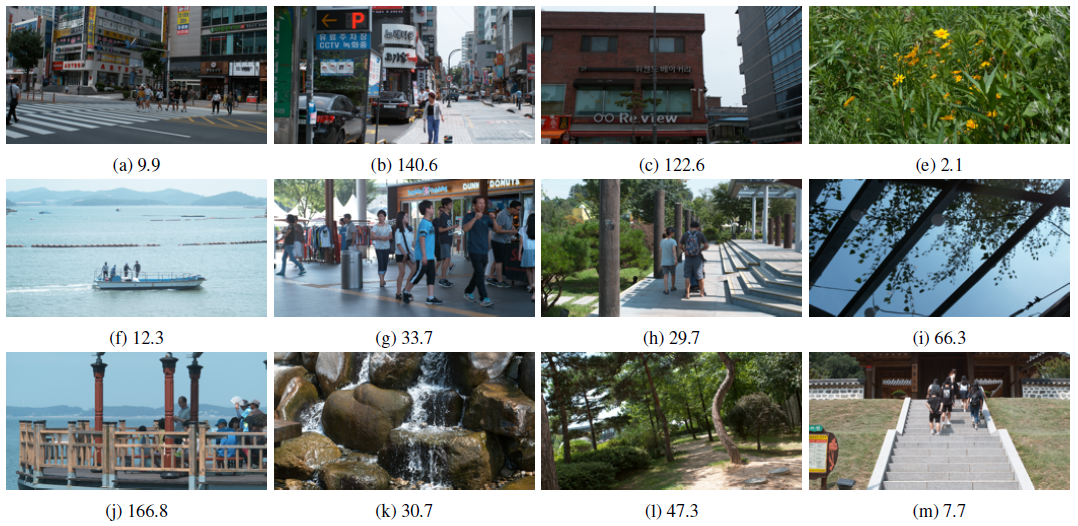
\includegraphics[width=0.7\linewidth]{images/dataset.png}
		\end{figure}
		\begin{itemize}
			\item Various objects: crowds, cars, trains, plants, boats$\cdots$
			\item Various places: stadiums, stations, beaches, rivers$\cdots$
		\end{itemize}
		}
		\only<2>{
			\begin{itemize}
				\item Impressive \alert{$4K@1000fps$} dataset.
			\end{itemize}
			\begin{figure}
				\centering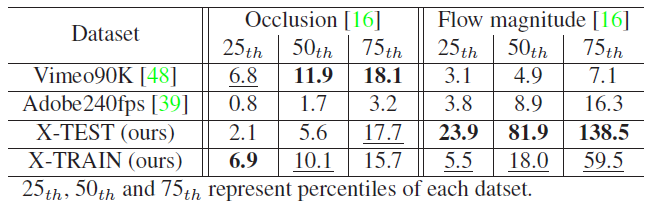
\includegraphics[width=0.6\linewidth]{images/dataset_analysis.png}
			\end{figure}
			\begin{itemize}
				\item Detailedly analysis: occlusion, flow magnitude
				\item Select extreme scenes for \alert{X-TRAIN} and \alert{X-TEST}.
			\end{itemize}
		}
	\end{frame}

	\begin{frame}{Proposed Method}
		\only<1>{
			\begin{itemize}
				\item Feature Extraction: strided conv $+$ residual block
			\end{itemize}
			\begin{figure}
				\centering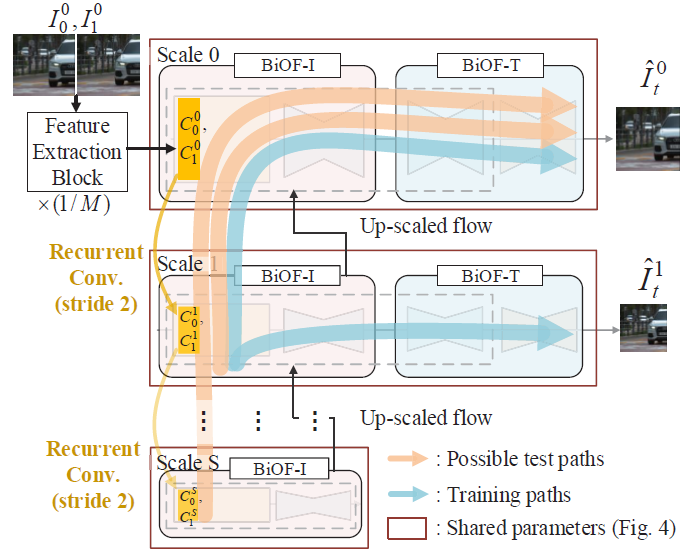
\includegraphics[width=0.6\linewidth]{images/all_structure.png}
			\end{figure}
			\begin{itemize}
				\item Scale Adaptivity: \alert{Shared} parameters, adapt to resolution of $I_0,\ I_1$ 
			\end{itemize}

		}
		\only<2-6>{
			\begin{itemize}
				\item Arch of XVFI-Net in scale \alert{s}.
			\end{itemize}
			\begin{figure}
				\centering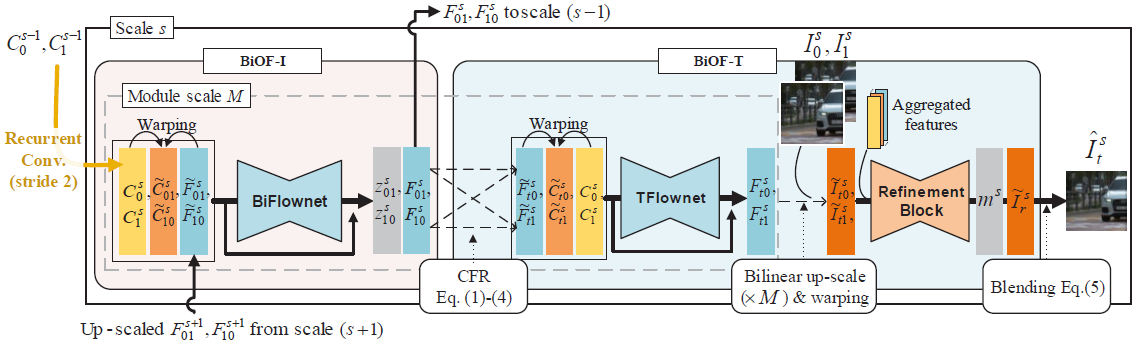
\includegraphics[width=0.95\linewidth]{images/scale_s.png}
			\end{figure}
		}
		\only<3>{
			\begin{itemize}
				\item BIOF-I module
				\begin{itemize}
					\item Input: context info $C^{s-1}_{0},\ C^{s-1}_{1}$, $s+1$-scale Flow $F^{s+1}_{01},\ F^{s+1}_{10}$
					\item Output: $s$-scale Flow  $F^{s}_{01},\ F^{s}_{10}$
				\end{itemize}
			\end{itemize}
		}
		\only<4>{
			\begin{itemize}
				\item BIOF-T module: 
				\begin{equation}
					\tilde{F}_{t 0}^{\mathrm{x}}=\frac{(1-t) \sum_{\mathcal{N}_{0}} w_{0} \cdot\left(-F_{0 t}^{\mathrm{y}}\right)+t \sum_{\mathcal{N}_{1}} w_{1} \cdot F_{1 \cdot(1-t)}^{\mathbf{y}}}{(1-t) \sum_{\mathcal{N}_{0}} w_{0}+t \sum_{\mathcal{N}_{1}} w_{1}}
				\end{equation}
				\begin{equation}
					\tilde{F}_{t 1}^{\mathrm{x}}=\frac{(1-t) \sum_{\mathcal{N}_{0}} w_{0} \cdot F_{0 .(1-t)}^{\mathrm{y}}+t \sum_{\mathcal{N}_{1}} w_{1} \cdot\left(-F_{1 t}^{\mathrm{y}}\right)}{(1-t) \sum_{\mathcal{N}_{0}} w_{0}+t \sum_{\mathcal{N}_{1}} w_{1}}
				\end{equation}
			\end{itemize}
		}
		\only<5>{
			\begin{itemize}
				\item BIOF-T module:
				\begin{equation}
					\mathcal{N}_{0}=\left\{\mathbf{y} \mid \text { round }\left(\mathbf{y}+F_{0 t}^{\mathbf{y}}\right)=\mathbf{x}\right\} \tag{3}
				\end{equation}
				\begin{equation}
					\mathcal{N}_{1}=\left\{\mathbf{y} \mid \text { round }\left(\mathbf{y}+F_{1 t}^{\mathbf{y}}\right)=\mathbf{x}\right\} \tag{4}
				\end{equation}
				\begin{equation}
					w_{i}=z_{i}^{\mathbf{y}} \cdot G\left(\left|\mathbf{x}-\left(\mathbf{y}+F_{i t}^{\mathbf{y}}\right)\right|\right) \tag{5}
				\end{equation}
				\begin{equation}
					G(d)=e^{-d^{2} / \sigma^{2}} \tag{6}
				\end{equation}
			\end{itemize}
		}
		\only<6>{
			\begin{itemize}
				\item BIOF-T module:
				\begin{equation*}
					\hat{I}_{t}^{s}=\frac{(1-t) \cdot m^{s} \cdot \tilde{I}_{t 0}^{s}+t \cdot\left(1-m^{s}\right) \cdot \tilde{I}_{t 1}^{s}}{(1-t) \cdot m^{s}+t \cdot\left(1-m^{s}\right)}+\tilde{I}_{r}^{s}
				\end{equation*}
			\end{itemize}
			\quad where $m^s$ is occlusion mask and $\tilde{I}_{r}^{s}$ is residual image.
		}
		\only<7>{
			\begin{figure}
				\centering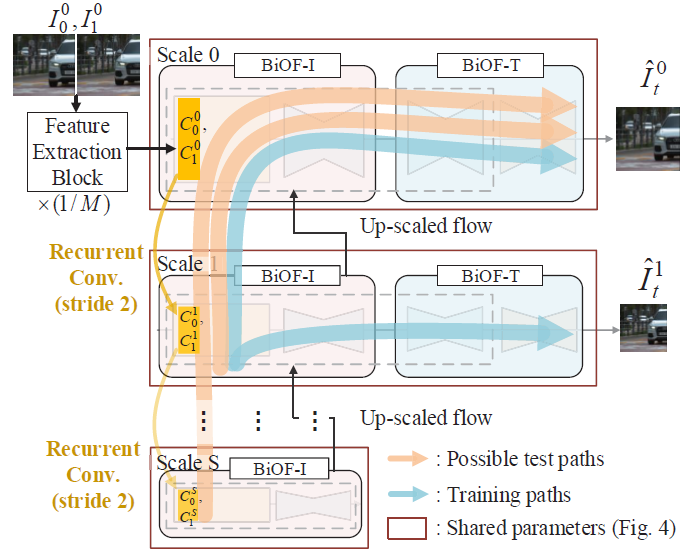
\includegraphics[width=0.5\linewidth]{images/all_structure.png}
			\end{figure}
			\begin{footnotesize}
			\begin{block}{Loss Function}
				\begin{itemize}
					\item $ \mathcal{L}_{\text {total }}=\mathcal{L}_{r}+\lambda_{s} \cdot \mathcal{L}_{s} $
					\item Multi-scale reconstruction loss: $ \mathcal{L}_{r}=\sum_{s=0}^{S_{t r n}}\left\|\hat{I}_{t}^{s}-I_{t}^{s}\right\|_{1} $
					\item Edge-aware smoothness loss: $\mathcal{L}_{s}=\sum_{i=0,1} \exp \left(-e^{2} \sum_{c}\left|\nabla_{\mathbf{x}} I_{t_{c}}^{0}\right|\right)^{\top} \cdot\left|\nabla_{\mathbf{x}} F_{t i}^{0}\right|$
				\end{itemize}
				
			\end{block}
			\end{footnotesize}
		}
	\end{frame}

	\begin{frame}{Model Analysis}
		\begin{columns}[c]
			\column{0.6\textwidth}
			\begin{itemize}
				\item {Shared parameters$\to$\alert{lightweighted}.}
				\item {Inference can start from any scale level.}
				\item {Coarse-to-fine strategy, but start from \alert{low spatial resolution}.}
				\item {Interpolate a frame at \alert{any time} instance from two input frames.}
			\end{itemize}\
			\column{0.5\textwidth}
			\begin{figure}
				\centering
				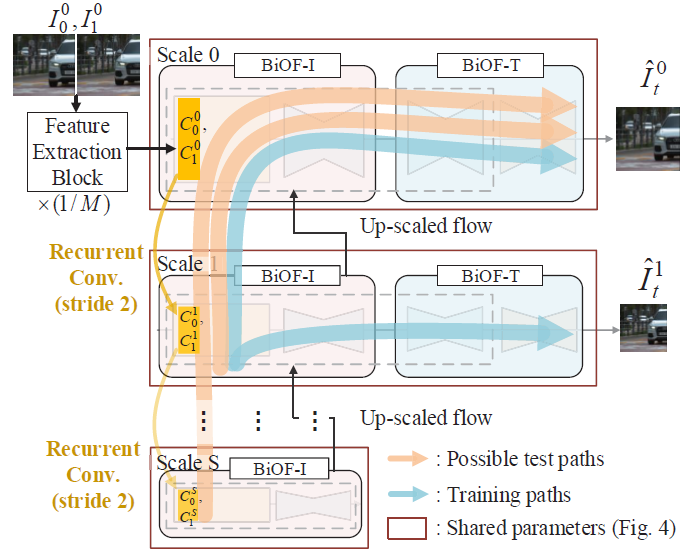
\includegraphics[width=6cm]{images/all_structure.png}
			\end{figure}
		\end{columns}
	\end{frame}

	\begin{frame}{Comparison to SOTA}
		\only<1-2>{
			\begin{itemize}
				\item Settings
				\begin{itemize}
					\item Retrain SOTA on X-TRAIN with sub $f$, original with sub $o$.
					\item XVFI-Net train($S_{trn}=3$) and test($S_{tst}=3\ or\ 5$).
				\end{itemize}
				\item Results:
			\end{itemize}
		}
		\only<1>{
			\begin{figure}
				\centering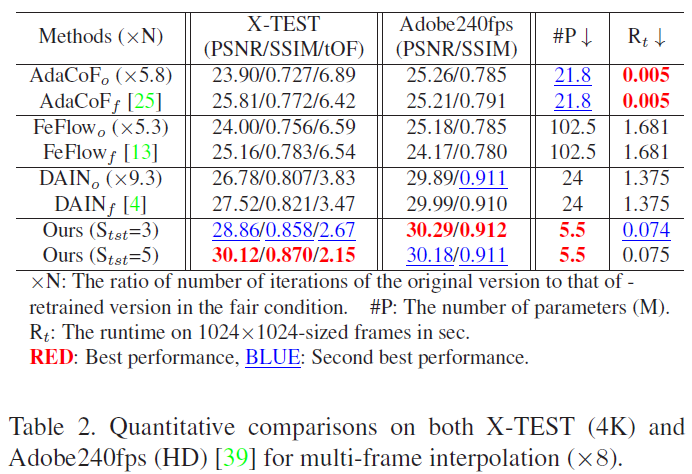
\includegraphics[width=0.6\linewidth]{images/data_result.png}
			\end{figure}
		}
		\only<2>{
			\begin{figure}
				\centering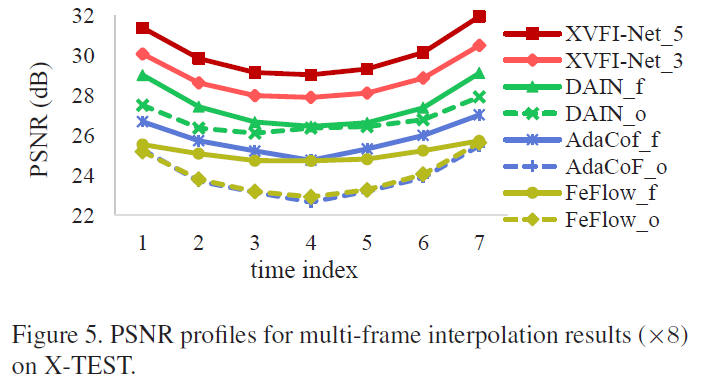
\includegraphics[width=0.6\linewidth]{images/PSNR_profile.png}
			\end{figure}
		}
		\only<3>{
			\begin{itemize}
				\item Qualitive Results:
			\end{itemize}
			\begin{figure}
				\centering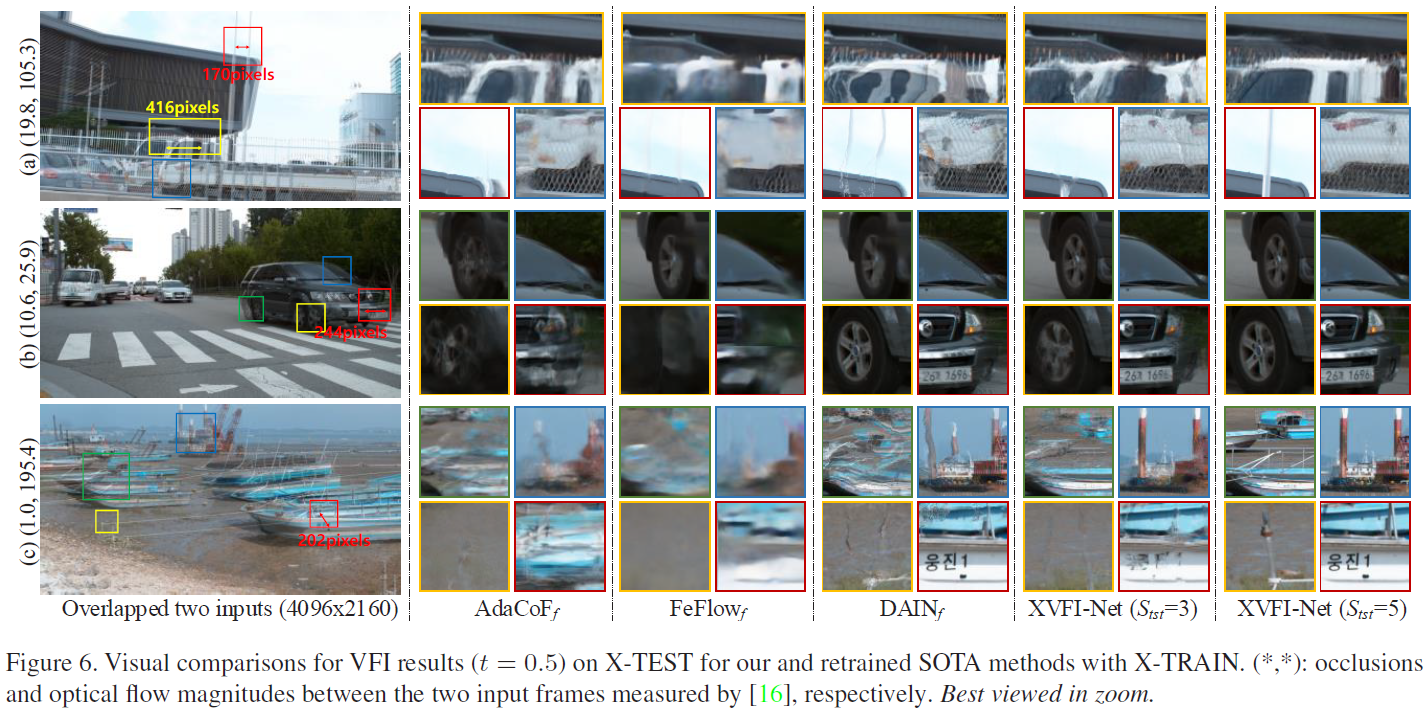
\includegraphics[width=0.9\linewidth]{images/Visual_results.png}
			\end{figure}
		}
	\end{frame}
	
	\begin{frame}{Ablation Studies}
		\only<1>{
			\begin{figure}
				\centering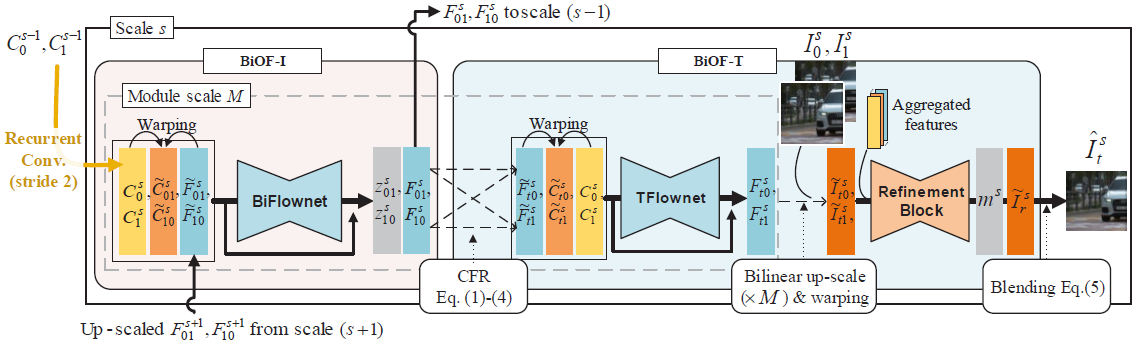
\includegraphics[width=0.9\linewidth]{images/scale_s.png}
			\end{figure}
		}
		\only<2>{
			\begin{itemize}
				\item Flow Approximation
			\end{itemize}
			\begin{figure}
				\centering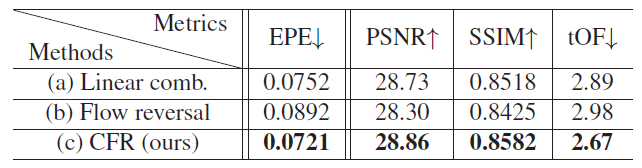
\includegraphics[width=0.7\linewidth]{images/FLOW_ABLATION.png}
			\end{figure}
			\begin{itemize}
				\item Adjustable scalability
				\begin{figure}
					\centering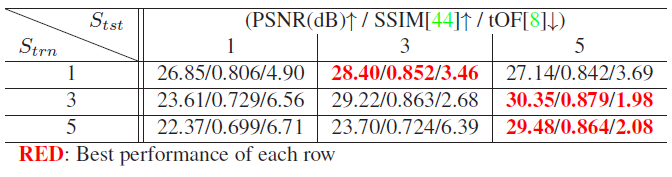
\includegraphics[width=0.7\linewidth]{images/adjustable_scalability.png}
				\end{figure}
			\end{itemize}
		}
		\only<3>{
			\begin{itemize}
				\item Robustness on LR-LFR dataset
				\bigskip
				\begin{figure}
					\centering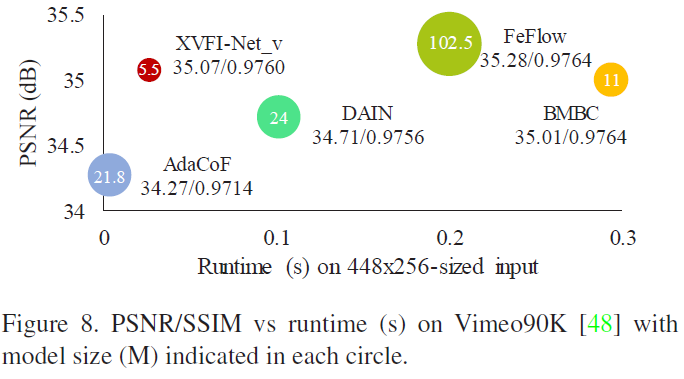
\includegraphics[width=0.6\linewidth]{images/robustness.png}
				\end{figure}
			\end{itemize}
		}
	\end{frame}

	\begin{frame}{Failure cases}
		\only<1>{
			\begin{itemize}
				\item Cases on 4K patches, with very large flow magnitude($ 196.5 $)
			\end{itemize}
			\begin{figure}
				\centering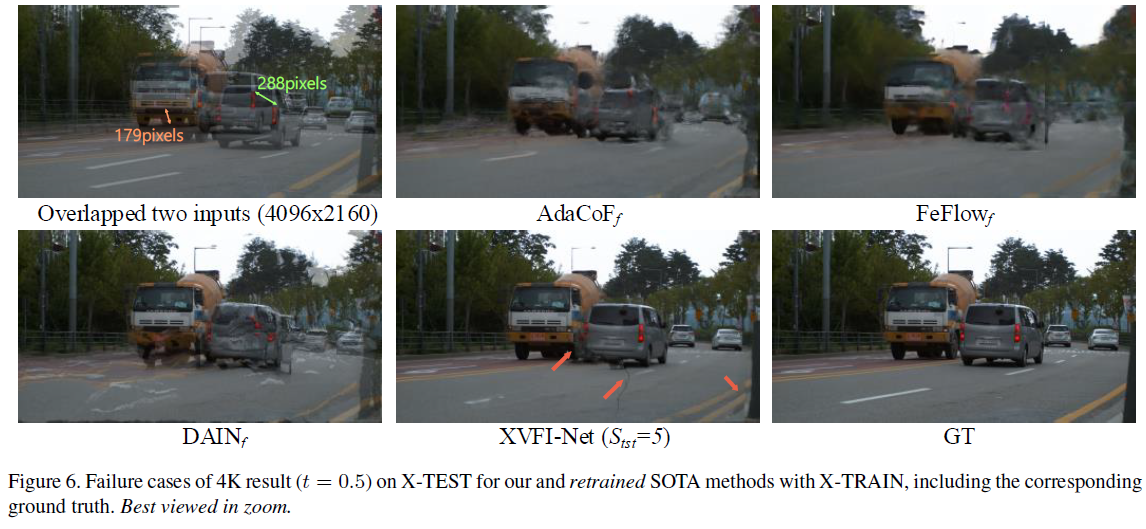
\includegraphics[width=0.9\linewidth]{images/case1.png}
			\end{figure}
		}
		\only<2>{
			\begin{itemize}
				\item Cases on croped patches
			\end{itemize}
			\begin{figure}
				\centering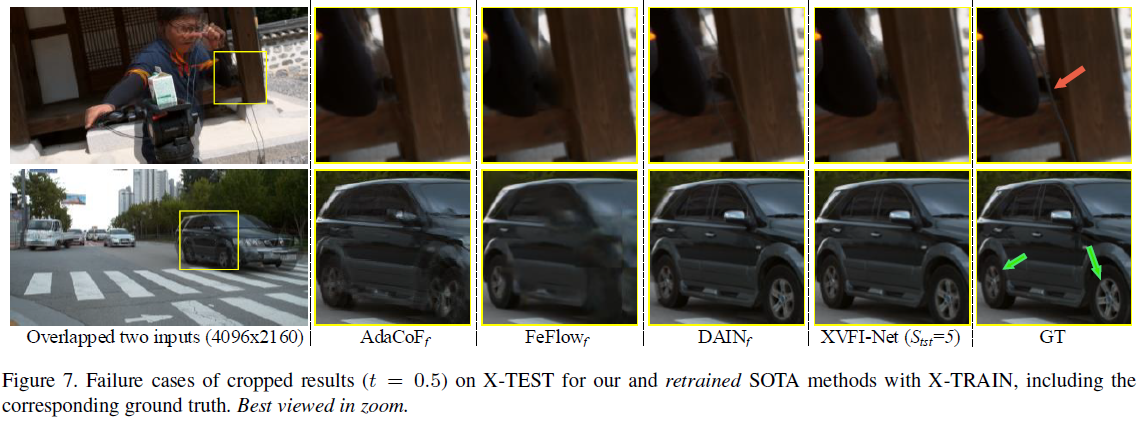
\includegraphics[width=0.9\linewidth]{images/case2.png}
			\end{figure}
			\begin{itemize}
				\item Analysis: attribute to flow and warping algorithm.
			\end{itemize}
			}
	\end{frame}
	
	\begin{frame}{Conclusion}
		\begin{itemize}
			\item Contributed HR-HFR \alert{X4K1000FPS} dataset is very \alert{valuable} for research.
			\item XVFI-Net showed \alert{SOTA} performance on HR dataset, also \alert{robust} to LR-LFR dataset.
			\item Extend VFI for more recent \alert{real-world applications} with HR video.
		\end{itemize}
	\end{frame}

	\begin{frame}{}
		\centering \Huge
		\emph{Thanks,  Q \& A }
	\end{frame}
\end{document}
